%% 
%% Copyright 2007, 2008, 2009 Elsevier Ltd
%% 
%% This file is part of the 'Elsarticle Bundle'.
%% ---------------------------------------------
%% 
%% It may be distributed under the conditions of the LaTeX Project Public
%% License, either version 1.2 of this license or (at your option) any
%% later version.  The latest version of this license is in
%%    http://www.latex-project.org/lppl.txt
%% and version 1.2 or later is part of all distributions of LaTeX
%% version 1999/12/01 or later.
%% 
%% The list of all files belonging to the 'Elsarticle Bundle' is
%% given in the file `manifest.txt'.
%% 

%% Template article for Elsevier's document class `elsarticle'
%% with numbered style bibliographic references
%% SP 2008/03/01

\documentclass[preprint,12pt, a4paper]{elsarticle}


%% The amssymb package provides various useful mathematical symbols
\usepackage{amssymb}

\usepackage[latin1]{inputenc}
\usepackage{amsmath}
\usepackage{listings}
\usepackage{marvosym}
\usepackage{color}
\usepackage{graphicx}
\usepackage{caption}
\usepackage{pgf}
\usepackage{tikz}
\usepackage{subfig}
\usepackage[american]{babel}
\usetikzlibrary{arrows,automata,positioning}
\usepackage{epstopdf}
\newtheorem{mydef}{Definition}
\newtheorem{mylem}{Lemma}
\usepackage{afterpage}

\renewcommand{\baselinestretch}{0.975}

\lstset{language=C,basicstyle=\tiny}
\lstset{numbers=left, numberstyle=\tiny, stepnumber=1, numbersep=5pt}
\lstset{tabsize=2}
\lstset{firstnumber=1}
\lstset{frame=single}
\lstset{
  language={C},
  morekeywords={enquanto,se,fim,entao,senao,retorne,faca,assume,then,end-if,end,input,output,cudaMemcpyHostToDevice,cudaMemcpyDeviceToHost,\_\_global\_\_}
}

\hyphenation{port-a-ble}

\newcommand{\comment}[1]{}

%% The lineno packages adds line numbers. Start line numbering with
%% \begin{linenumbers}, end it with \end{linenumbers}. Or switch it on
%% for the whole article with \linenumbers.
\usepackage{lineno}

\journal{Science of Computer Programming}

\begin{document}

\begin{frontmatter}


\title{ESBMC-GPU \\ A Context-Bounded Model Checking Tool \\ to Verify CUDA Programs}

\author{Felipe~R.~Monteiro$^{1}$, Erickson~H.~da~S.~Alves$^{1}$, Isabela~S.~Silva$^{1}$,\\Hussama~A.~Ismail$^{1}$, Lucas~C.~Cordeiro$^{1,2}$, and Eddie~B.~de~Lima~Filho$^{1,3}$}

\address{$^{1}$Faculty of Technology, Federal University of Amazonas, Brazil \\ 
$^{2}$Department of Computer Science, University of Oxford, United Kingdom \\
$^{3}$ FPF Tech, Brazil}

\begin{abstract}
The Compute Unified Device Architecture (CUDA) is a programming model used for exploring the advantages of Graphics Processing Unit (GPU) devices, through parallelization and specialized functions and features. Nonetheless, as in other development platforms, errors may occur, due to traditional software creation processes, which may even compromise the execution of an entire system. In order to address such a problem, ESBMC-GPU was developed, as an extension to the Efficient SMT-Based Context-Bounded Model Checker (ESBMC). In summary, ESBMC processes input code through ESBMC-GPU and an abstract representation of the standard CUDA libraries, with the goal of checking a set of desired properties. Experimental results showed that ESBMC-GPU was able to correctly verify $85$\% of the chosen benchmarks and it also overcame other existing GPU verifiers.
\end{abstract}

\begin{keyword}
GPU verification \sep formal verification \sep model checking \sep CUDA

\end{keyword}

\end{frontmatter}

\linenumbers

%=-=-=-=-=-=-=-=-=-=-=-=-=-=-=-=-=-=-=-=-=-=-=-=-=-=-=
\section{Introduction} 
\label{sec:intro}
%=-=-=-=-=-=-=-=-=-=-=-=-=-=-=-=-=-=-=-=-=-=-=-=-=-=-=

The Compute Unified Device Architecture (CUDA) is a development framework that makes use of the architecture and processing power of Graphics Processing Units (GPUs)~\cite{cuda:2012}. Indeed, CUDA is also an Application Programming Interface (API), through which a GPU's parallelization scheme and tools can be accessed, with the goal of executing kernels. Nonetheless, source code is still written by human programmers, which may result in arithmetic overflow, division by zero, and other violation types. In addition, given that CUDA allows parallelization, problems related to the latter can also occur, due to thread scheduling~\cite{betts:2012}.

In order to address the mentioned issues, an extension to the Efficient SMT-Based Context-Bounded Model Checker (ESBMC)~\cite{cordeiro:2012} was developed, named as ESBMC-GPU~\cite{Pereira15,Pereira16,pereira:2016}, with the goal of verifying CUDA-based programs (available online at \texttt{http://esbmc.org/gpu}). ESBMC-GPU consists of an extension for parsing CUDA source code ({\it i.e.}, a front-end to ESBMC) and a CUDA operational model (COM), which is an abstract representation of the standard CUDA libraries ({\it i.e.}, the native API) that conservatively approximates their semantics. 

A distinct feature of ESBMC-GPU, when compared with other approaches \cite{betts:2012,Li:2010,Li:2012,civl:2015}, is the use of Bounded Model Checking (BMC)~\cite{Biere:2009} allied to Satisfiability Modulo Theories (SMT)~\cite{Barrett:2009}, with explicit \textcolor{blue}{state-space exploration}~\cite{cordeiro:2011,cordeiro:2012}. In summary, concurrency problems are tackled, up to an unwinding bound, while each interleaving itself is symbolically handled; however, even with BMC, state-space exploration may become a very time-consuming task, which is alleviated through state hashing and Monotonic Partial Order Reduction (MPOR)~\cite{KahlonWG09}. As a consequence, redundant interleavings are eliminated, without ignoring a program's behavior.

Finally, existing GPU verifiers often ignore some aspects related to memory leak, data transfer, and overflow, which are normally present in CUDA programs. The proposed approach, in turn, explicitly addresses them, through an accurate checking procedure, which even considers data exchange between main program and kernel. Obviously, it results in higher verification times, but more errors can then be identified and later corrected, in another development cycle.

%=-=-=-=-=-=-=-=-=-=-=-=-=-=-=-=-=-=-=-=-=-=-=-=-=-=-=
%\subsection{Existing GPU Verifiers}
%\label{sec:related-work}
%=-=-=-=-=-=-=-=-=-=-=-=-=-=-=-=-=-=-=-=-=-=-=-=-=-=-=

%\textbf{Existing GPU Verifiers}. GPUVerify~\cite{betts:2012} is based on Synchronous Delayed Visibility, which focus on detecting data race and barrier divergence, while reducing kernel verification procedures to the analysis of sequential programs. Symbolic Executor with Static Analysis (SESA)~\cite{sesa:2014} and GPU + KLEE (GKLEE)~\cite{Li:2012} are concrete plus symbolic (\textit{concolic}) execution tools. Initially, GKLEE modeled every original thread, which was later improved by taking into account symmetry, and it considers both kernel and main function, while checking barrier synchronization and data race, among others. SESA combines equivalent flows, which results in great performance improvement, focus on data race detection, and does not verify the main function. Prover of User GPU Programs (PUG)~\cite{Li:2010} is based on SMT solvers and applies symbolic static analysis to each kernel, but requires user annotations. CIVL~\cite{civl:2015} generates an abstract syntax tree and supports analysis and transformations. Besides, it also verifies concurrent programs with partial order reduction, which makes it very similar to the solution proposed here. Given that its support to CUDA libraries is still under development, CIVL is an interesting approach for checking simple CUDA programs. \textcolor{red}{$<$---- poderiamos deletar esse paragrafo?}

%=-=-=-=-=-=-=-=-=-=-=-=-=-=-=-=-=-=-=-=-=-=-=-=-=-=-=
\section{Architecture and Implementation}
\label{sec:arch}
%=-=-=-=-=-=-=-=-=-=-=-=-=-=-=-=-=-=-=-=-=-=-=-=-=-=-=

\textcolor{blue}{ESBMC-GPU is built on top of ESBMC}, which is an open source context-bounded model checker based on SMT solvers for \textcolor{blue}{ANSI-C/C$++$ programs~\cite{cordeiro:2011, cordeiro:2012, ramalho:2013}}, and adds four essential models, as described below.

\begin{figure}[htb]
  \centering
  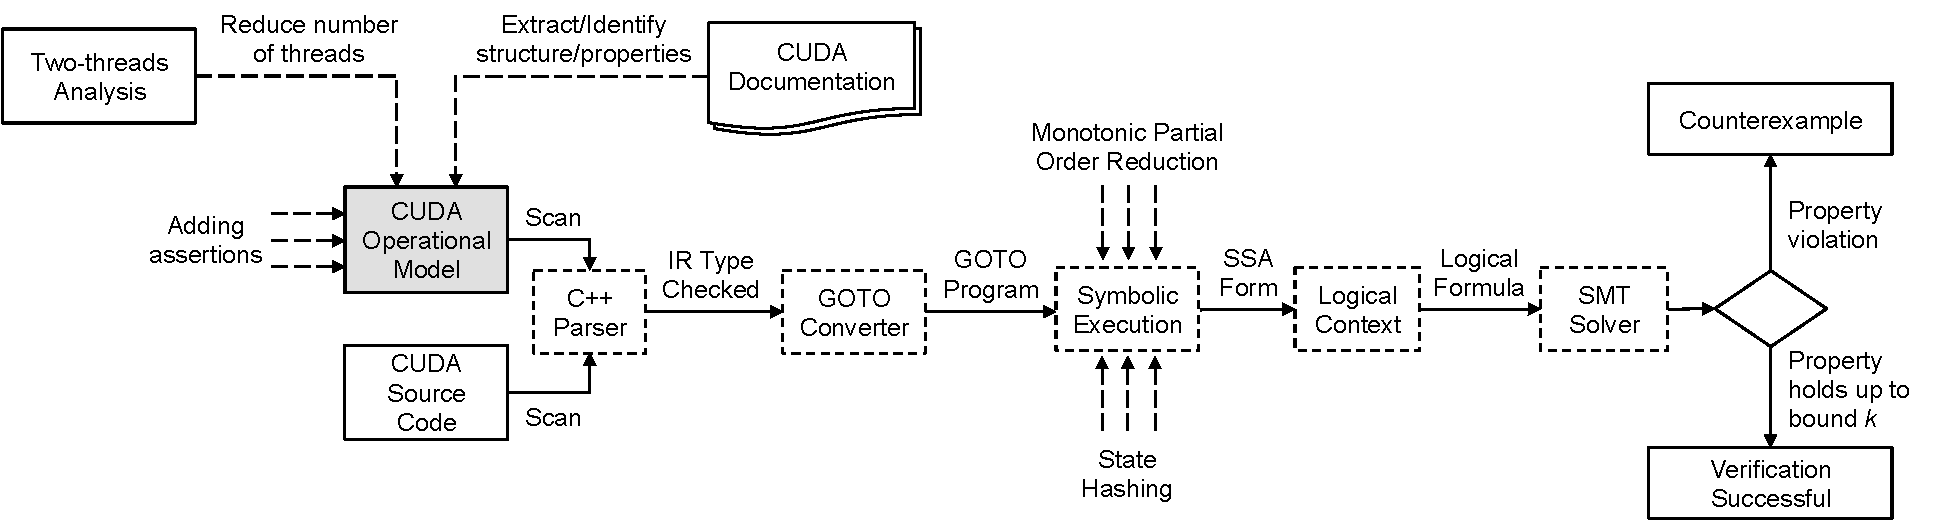
\includegraphics[width=5.5in]{../figures/arch.pdf}
  \caption{Overview of ESBMC-GPU's architecture.}
  \label{figure:arch}
\end{figure}

\noindent \textbf{1. CUDA Operational Model.} An operational model for CUDA libraries that provides support to CUDA functionalities, in conjunction with ESBMC, as shown in Fig.~\ref{figure:arch}. Such an approach, which was previously attempted in the verification of C++ programs~\cite{ramalho:2013, monteiro:2015, garcia:2016, monteiro:2017}, \textcolor{blue}{consists of} an abstract representation that reliably approximates the CUDA library's semantics; however, COM incorporates pre- and post-conditions into verification processes, which enables ESBMC-GPU to verify specific properties (cf. Sec.~\ref{sec:features}). Indeed, COM allows the necessary control for performing code analysis, where both CUDA operation and knowledge for model checking its properties are available.

%\begin{figure}[htb]
%  \centering
%  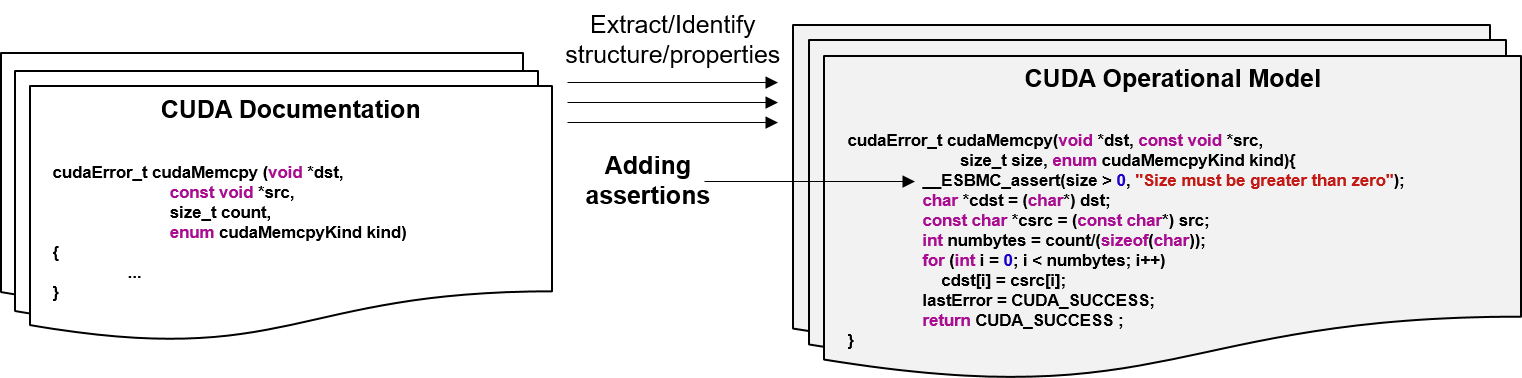
\includegraphics[width=4.5in]{../figures/cuda-om.png}
%  \caption{CUDA operational model development process.}
%  \label{figure:om}
%\end{figure}

ESBMC was designed to handle multi-threaded software, through the use of an API called Portable Operating System Interface (POSIX -- ISO/IEC 9945)~\cite{posix:2008}. Thus, ESBMC-GPU applies a combination of processing methods used by Central Processing Units (CPUs) and the POSIX library, where thread instructions can interleave to create execution paths. Particularly, COM simulates the behavior of kernel calls using pthread functions ({\it e.g.}, {\tt pthread\_create}) and combines that with ESBMC, in order to check data race and specific C/C++ programming language failures ({\it e.g.}, array out-of-bounds and pointer safety).\\

\noindent \textbf{2. Two-threads Analysis.} Similarly to GPUVerify~\cite{betts:2012} and PUG~\cite{Li:2010}, ESBMC-GPU also reduces the number of threads (to only two elements), during the verification of CUDA programs, by considering a NVIDIA Fermi GPU architecture, in order to improve verification time and avoid the state-space explosion problem. In CUDA programs, whilst threads execute the same parametrized kernel, only two of them are necessary for conflict check. Thus, such an analysis ensures that errors ({\it e.g.}, data races) detected between two threads, in a given subgroup and due to unsynchronized accesses to shared variables, are enough to justify a property violation~\cite{pereira:2016}.\\

\noindent \textbf{3. State Hashing.} ESBMC-GPU applies state hashing to further eliminate redundant interleavings and also \textcolor{blue}{reduce the state space}, based on SHA256 hashes \cite{FIPS:2002}. In particular, its symbolic state hashing approach computes a summary for a particular state that has already been explored and then indexes the resulting set, in order to reduce the generation of redundant states. Given any state computed during the symbolic execution of a specific CUDA kernel, ESBMC-GPU simply summarizes it and efficiently determines whether it has been explored before or not, along a different computation path. When this behavior is confirmed, which happens during the ESBMC-GPU's symbolic-execution procedure, then the current computation path does not need to be further explored in the associated reachability tree (RT). This way, if ESBMC-GPU reaches such a state, {\it i.e.}, where a context switch can be taken ({\it e.g.}, before a global variable or synchronization primitive) and all shared/local variables and program counters are similar to another explored node, then ESBMC-GPU just considers that an identical node to be further explored, since reachability subtrees associated to them are also similar~\cite{pereira:2016,morse:2015}.\\

\noindent \textbf{4. Monotonic Partial Order Reduction.} MPOR is used to reduce the number of thread interleavings, by classifying transitions inside a program as dependent or independent. As a consequence, it is possible to determine whether interleaving pairs always lead to the same state and then remove duplicates in a reachability tree, without ignoring any program's behavior~\cite{morse:2015}.

%=-=-=-=-=-=-=-=-=-=-=-=-=-=-=-=-=-=-=-=-=-=-=-=-=-=-=
\section{Functionalities}
\label{sec:features}
%=-=-=-=-=-=-=-=-=-=-=-=-=-=-=-=-=-=-=-=-=-=-=-=-=-=-=

%Through the integration of COM into ESBMC ({\it i.e.}, ESBMC-GPU), one is able to analyze CUDA programs and verify the following properties: data-race conditions, in order to detect if multiple threads perform unsynchronized access \textcolor{blue}{to the same memory locations}; pointer safety, {\it i.e.}, whether {\it (i)} a pointer offset does not exceed object bounds and {\it (ii)} a pointer is neither {\tt NULL} nor invalid; array bounds, in order to ensure that array indices are within known bounds; arithmetic under- and overflow, which happens when a sum or product exceeds the memory limits that a variable can handle; division by zero, which takes place when denominators, in arithmetic expressions, lead to a division by zero; and user-specified assertions, {\it i.e.}, all assertions specified by users, which is essential to a thorough verification process.%, as some specific possible violations must be explicitly pointed out.

%In order to check the aforementioned properties, ESBMC-GPU explicitly explores the possible interleavings (up to the given context bound) and calls the single-threaded BMC procedure on each one, whenever it reaches an RT leaf node. Then, the mentioned procedure will stop if it finds a bug or when all possible RT interleavings \textcolor{blue}{have been systematically explored}~\cite{pereira:2016}.


\textcolor{blue}{Through the integration of COM into ESBMC ({\it i.e.}, ESBMC-GPU), one is able to analyze CUDA programs and verify the following properties:}

\begin{itemize}
	\item[--] \textcolor{blue}{\textbf{Data race.} ESBMC-GPU checks data race conditions, in order to detect if multiple threads perform unsynchronized access \textcolor{blue}{to the same memory locations};}
	
	\item[--] \textcolor{blue}{\textbf{Pointer safety.} ESBMC-GPU also ensures that {\it (i)} a pointer offset does not exceed object bounds and {\it (ii)} a pointer is neither {\tt NULL} nor invalid;}
	
	\item[--] \textcolor{blue}{\textbf{Array bounds.} ESBMC-GPU performs array-bound checking, in order to ensure that any variable, used as an array index, is within known bounds;}
	
	\item[--] \textcolor{blue}{\textbf{Arithmetic under- and overflow.} ESBMC-GPU checks whether a sum or product exceeds the memory limits that a variable can handle, which can cause an error capable of spreading through the entire execution path;}
	
	\item[--] \textcolor{blue}{\textbf{Division by zero.} ESBMC-GPU analyzes whether denominators, in arithmetic expressions, lead to a division by zero;}
	
	\item[--] \textcolor{blue}{\textbf{User-specified assertions.\ } ESBMC-GPU considers all assertions specified by users, which is essential to a thorough verification process, as some specific possible violations must be explicitly pointed out.}
\end{itemize}

In order to check the aforementioned properties, ESBMC-GPU explicitly explores the possible interleavings (up to the given context bound) and calls the single-threaded BMC procedure on each one, whenever it reaches an RT leaf node. Then, the mentioned procedure will stop if it finds a bug or when all possible RT interleavings \textcolor{blue}{have been systematically explored}~\cite{pereira:2016}. \textcolor{blue}{Furthermore, ESBMC-GPU has the following additional command-line options:
\\
\texttt{--no-assertions}: to ignore assertions; \\
\texttt{--no-bounds-check}: to skip array bounds check; \\
\texttt{--no-div-by-zero-check}: to skip division by zero check; \\
\texttt{--no-pointer-check}: to skip pointer check; \\
\texttt{--memory-leak-check}: to enable memory leak check; \\
\texttt{--overflow-check}: to enable arithmetic over- and underflow check; \\
\texttt{--deadlock-check}: to enable global and local deadlock check with mutex; \\
\texttt{--data-races-check}: to enable data races check; \\
\texttt{--lock-order-check}: to enable for lock acquisition ordering check; \\
\texttt{--atomicity-check}: to enable atomicity check at visible assignments; \\
\texttt{--memlimit}: to configure memory limit, of form ``100MB'' or ``2GB''; \\
\texttt{--timeout}: to configure time limit, integer followed by \{s, m, or h\}; \\
\texttt{--force-malloc-success}: to consider that there is always enough memory available in the device; \\
\texttt{-DGPU\_threads=<$number$>}: to define the total number of threads by kernel. \\}

%=-=-=-=-=-=-=-=-=-=-=-=-=-=-=-=-=-=-=-=-=-=-=-=-=-=-=
\section{Illustrative Example}
\label{subsec:usage}
%=-=-=-=-=-=-=-=-=-=-=-=-=-=-=-=-=-=-=-=-=-=-=-=-=-=-=

In this part, ESBMC-GPU usage is demonstrated, by using the CUDA program shown in Fig.~\ref{fig:illustrative-example}. First of all, users must replace the default kernel call (line $16$) by an intrinsic function of ESBMC-GPU (line $17$). Then, the resulting CUDA program can be passed to the command-line version of ESBMC-GPU, as follows: %\texttt{esbmc-gpu} \emph{\tt <file>.cu} {\tt --unwind <$k$>}  {\tt --context-switch <$c$>} {\tt --state-hashing} {\tt -I <path-to-CUDA-OM>},  

\begin{center}
\noindent \texttt{esbmc-gpu} \emph{\tt <file>.cu} {\tt --unwind <$k$>}  {\tt --context-switch <$c$>}

\noindent {\tt --state-hashing} {\tt -I <path-to-CUDA-OM>},
\end{center}

where {\tt $<$file$>$.cu} is the CUDA program, {\tt <$k$>} is the maximum loop unrolling, {\tt <$c$>} is a context-switch bound, {\tt --state-hashing} reduces redundant interleavings, and {\tt $<$path-to-} {\tt CUDA-OM$>$} is the location of the COM library.

%As one may see in Fig.~\ref{fig:illustrative-example}, this CUDA-based program has 1 block and 2 threads, and a kernel (lines $12$ to $14$), which assigns thread's index values to an array passed as an input argument. Indeed, its goal is to instantiate array positions according to the thread index. However, there is a mistake in the array index, as the value $1$ is accidentally added to the thread index (line $13$). As shown in the main function, array positions are assigned with value $0$ (line $23$), and after the kernel call (line $26$), it is expected that $a[0] == 0$ and $a[1] == 1$.

In the mentioned example, ESBMC-GPU detects an array out-of-bounds violation. Indeed, this CUDA-based program retrieves a memory region that has not been previously allocated, {\it i.e.}, when {\tt threadIdx.x = 1}, the program tries to access $a[2]$. Importantly, the {\tt cudaMalloc()} function's operational model has a precondition that checks if the memory size to be allocated is greater than zero. In addition, an assertion checks if the result matches to the expected postcondition (line $19$). The verification of this program through ESBMC-GPU produces $54$ successful and $3$ failed interleavings. For instance, one possible failed interleaving is represented by the threads executions $t_0 : a[1] = 0$; $t_1 : a[2] = 1$, where $a[2] = 1$ represents an incorrect access to the array index $a$. It is worth noticing that CIVL, ESBMC-GPU, and GKLEE are also able to detect this array out-of-bounds violation, but GPUVerify fails, as it reports a true incorrect result (missed bug).

\begin{figure} [htb]
\centering
\begin{minipage}{8.5cm}
\begin{lstlisting}
#include <...>
#define BLOCKS 1
#define THREADS 2

__global__ void kernel(int *A) {
	A[threadIdx.x + 1] = threadIdx.x;
}

int main(){
	int *a;
	int *dev_a;
	int size = THREADS*sizeof(int);
	a = (int*)malloc(size);
	cudaMalloc((void**)&dev_a, size);
	for (int i = 0; i < THREADS; i++)
		a[i] = 0;
	cudaMemcpy(dev_a, a, size, cudaMemcpyHostToDevice);
	// kernel<<<BLOCKS,THREADS>>>(dev_a);
	ESBMC_verify_kernel(kernel, BLOCKS, THREADS, dev_a);
	cudaMemcpy(a, dev_a , size , cudaMemcpyDeviceToHost);
	for (int i = 0; i < THREADS; i++)
		assert(a[i]==i);	
	cudaFree(dev_a);
	free(a);
	return 0;
}
\end{lstlisting}
\end{minipage}
\caption{Illustrative CUDA code example.}
\label{fig:illustrative-example}
\end{figure}

%=-=-=-=-=-=-=-=-=-=-=-=-=-=-=-=-=-=-=-=-=-=-=-=-=-=-=
\section{Experimental Evaluation}
\label{sec:effectiveness}
%=-=-=-=-=-=-=-=-=-=-=-=-=-=-=-=-=-=-=-=-=-=-=-=-=-=-=

In order to evaluate ESBMC-GPU's precision and performance, benchmarks\footnote{A detailed description of all benchmarks is available at {\tt http://esbmc.org/gpu/}} were extracted from the available literature ({\it i.e.}, NVIDIA GPU Computing SDK v$2$.$0$~\cite{toolkit:2015} and Microsoft C$++$ AMP Sample Projects~\cite{microsoft:2012}), which covers basic functions commonly used by real CUDA applications. 
%The chosen benchmark suite comprises $20$ CUDA kernels from NVIDIA GPU Computing SDK v$2$.$0$, $20$ CUDA kernels from Microsoft C$++$ AMP Sample Projects%~\cite{microsoft:2012}
%, and $104$ CUDA-based programs that explore a wide range of CUDA functionalities~\cite{cuda:2012}. In summary, the chosen suite contains $47.4$\% bug-free and $52.6$\% buggy benchmarks, which tackle data race, arithmetic operations, pointer assignment, {\tt \_\_device\_\_} function calls, general ANSI-C functions ({\it e.g.}, \texttt{memset}), general CUDA functions ({\it e.g.}, \texttt{cudaMemcpy}), general libraries in CUDA ({\it e.g.}, \texttt{curand.h}), and the ability to work with variables, type modifiers ({\it e.g.}, \texttt{unsigned}), pointers, type definitions, and intrinsic CUDA variables ({\it e.g.}, \texttt{uint4}) \textcolor{red}{poderiamos colocar toda essa descri��o dos benchmarks numa pagina online e cita-la aqui??}.
The present experiments answer two research questions: {\it (i)} How accurate is ESBMC-GPU when verifying the chosen benchmarks? {\it (ii)} How does ESBMC-GPU's performance compare to other existing verifiers?

%\begin{enumerate}

%\item {\bf (sanity check)} Which results does ESBMC-GPU obtain upon verifying benchmarks from the automated test suite?
%\item How accurate is ESBMC-GPU when verifying the chosen test suite?

%\item {\bf (compare software performance)} What is ESBMC-GPU performance when compared to GKLEE, GPUVerify, PUG, and CIVL?
%\item How does ESBMC-GPU compare to other existing verifiers?

%\end{enumerate}

 In order to answer both questions, all benchmarks were verified with $4$ GPU verifiers (ESBMC-GPU $v2.0$, GKLEE $v2012$, GPUVerify $v1811$, and CIVL $v1.7.1$), on an otherwise idle Intel Core i$7$-$4790$ CPU $3$.$60$ GHz, with $16$ GB of RAM, running Ubuntu 14.04 OS. Importantly, all presented execution times are actually CPU times, {\it i.e.}, only the elapsed time periods spent in the allocated CPUs, which was measured with the {\tt times} system call (POSIX system). An overview of the experimental results is shown in Fig.~\ref{figure:experimental}, where {\it True} represents bug-free benchmarks, {\it False} represents buggy benchmarks, {\it Not supported} represents benchmarks that could not be verified, {\it Correct} represents the percentage of benchmarks correctly verified, and {\it Incorrect} represents the percentage of benchmarks incorrectly verified ({\it i.e.}, a verification tool reports an unexpected result). As one may notice, the present experimental results show that ESBMC-GPU reached a successful verification rate of approximately $85\%$, while GKLEE, GPUVerify, and CIVL reported $72\%$, $50\%$, and $35\%$, respectively\footnote{All experimental results are available at {\tt http://esbmc.org/gpu/}}. More precisely, ESBMC-GPU supports the verification of benchmarks related to array bounds ($3$\%), assertive statements ($5$\%), data race ($11$\%), {\tt NULL} pointers ($3$\%), and other specific CUDA functionalities ($63$\%).\\

\begin{figure}[htb]
  \centering
  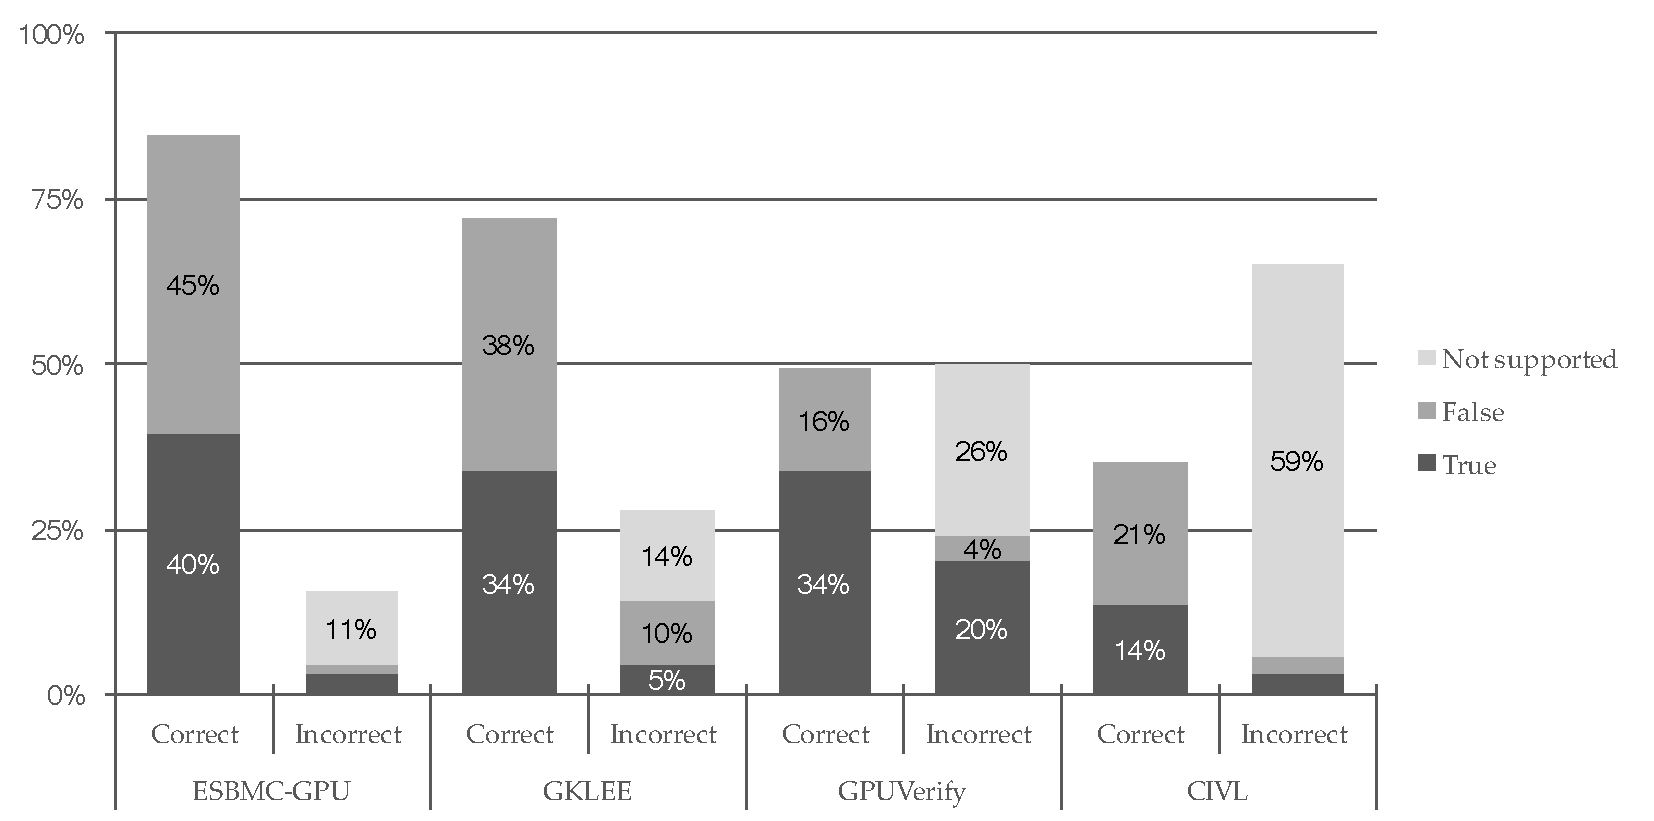
\includegraphics[width=4.5in]{../figures/experimental-results.pdf}
  \caption{Experimental evaluation of ESBMC-GPU against other verifiers.}
  \label{figure:experimental}
\end{figure}

{\bf Limitations.} ESBMC-GPU was unable to correctly verify $24$ benchmarks, which are related to constant memory access ($2$\%), CUDA's specific libraries ($4.5$\%), and the use of pointers to functions, structures, and {\tt char} type variables, when passed as kernel call arguments ($4.5$\%). In addition, it only reported $3$\% of incorrect true and $1$\% of incorrect false results.\\

{\bf Performance.} MPOR resulted in a performance improvement of approximately $80\%$, by decreasing the verification time from $16$ to $3$ hours, while the two-threads analysis further reduced that to $789.6$ sec. Although such techniques have considerably improved the ESBMC-GPU's performance, it still takes longer than the other evaluated tools: GPUVerify ($98.36$ sec), GKLEE ($108.32$ sec), and CIVL ($708.52$ sec). \textcolor{blue}{On the one hand}, this is due to thread interleavings, which combine symbolic model checking with explicit state-space exploration~\cite{pereira:2016}. %In addition, even though ESBMC-GPU reports the highest verification time, it still presents the highest accuracy, with less than $6$ seconds per benchmark.%, which shows that it is a feasible tool regarding the verification of CUDA-based applications. 
\textcolor{blue}{On the other hand}, ESBMC-GPU still presents the highest accuracy, with less than $6$ seconds per benchmark.

%\noindent \textbf{Availability of Data and Tools.} The performed experiments are based on a set of publicly available benchmarks. All benchmarks, tools, and results, associated with the current evaluation, are available on {\tt http://esbmc-gpu.org/}.

%=-=-=-=-=-=-=-=-=-=-=-=-=-=-=-=-=-=-=-=-=-=-=-=-=-=-=
\section{Conclusions and Future Work}
\label{sec:conc}
%=-=-=-=-=-=-=-=-=-=-=-=-=-=-=-=-=-=-=-=-=-=-=-=-=-=-=

ESBMC-GPU marks the first application of an SMT-based context-BMC tool that recognizes CUDA directives~\cite{pereira:2016}. \textcolor{blue}{Besides, it also applies MPOR, two-thread analysis, and state hashing in order to further simplify verification models and provides fewer incorrect results, compared with GKLEE, GPUVerify, and CIVL.} Finally, it presents improved ability to detect array out-of-bounds and data race violations. Future work aims to support \textcolor{blue}{CUDA (parallel) streams and events~\cite{cuda:2012}} and implement further techniques \textcolor{blue}{(e.g., Abstract Interpretation~\cite{Rocha2017}) in order to prune the state space exploration}, by taking into account GPU symmetry.

%\noindent \textbf{Acknowledgements.} This paper is based on research sponsored by the Institute of Development and Technology (INdT) and by the National Council for Scientific and Technological Development (CNPq) under agreement number $475647/2013-0$.

\section*{References}
\label{}

\begin{thebibliography}{25}

\bibitem{cuda:2012}
Cheng, J., Grossman, M., and McKercher, T.
\newblock {\em {Professional CUDA C Programming}}.
\newblock {John Wiley and Sons, Inc.} 2014.

%\bibitem{gpu:2010}
%Kirk, D. and Hwu, W.
%\newblock {\em {Programming Massively Parallel Processors}}.
%\newblock Elsevier, 2010.

\bibitem{betts:2012}
Betts, A., Chong, N., Donaldson, A., Qadeer, S., and Thomson, P.
\newblock {\em{GPUVerify: A Verifier for {GPU} Kernels}}.
\newblock {OOPSLA} 2012; 113--132.

\bibitem{cordeiro:2011}
Cordeiro, L. and Fischer, B.
\newblock {\em{Verifying Multi-threaded Software using SMT-based Context-Bounded
  Model Checking}}.
\newblock {ICSE} 2011; 331--340.

\bibitem{cordeiro:2012}
Cordeiro, L. and, Fischer, B., and Marques{-}Silva, J.
\newblock {\em{SMT-Based Bounded Model Checking for Embedded {ANSI-C} Software}}.
\newblock {IEEE} Trans. Software Eng. 2012; 38(4):957--974.

\bibitem{ramalho:2013}
\textcolor{blue}{Ramalho, M., Freitas, M., Sousa, F., Marques, H., Cordeiro, L., and Fischer, B.}
\newblock \textcolor{blue}{{\em{SMT-Based Bounded Model Checking of C++ Programs}}.}
\newblock \textcolor{blue}{Proceedings of the $20^{th}$ Annual IEEE International Conference and Workshops on the Engineering of Computer Based Systems, ECBS'13.}
\newblock \textcolor{blue}{{IEEE} Computer Society: Washington, DC, USA, 147--156, 2013.}

\bibitem{Pereira15}
Pereira, P., Albuquerque, H., Marques, H., Silva, I., Carvalho, C., Santos, V., Ferreira, R., and Cordeiro, L.
\newblock {\em{Verifica\c{c}\~ao de Kernels em Programas CUDA usando Bounded Model Checking.}} 
\newblock {WSCAD-SSC} 2015; 24--35.

\bibitem{Pereira16}
Pereira, P., Albuquerque, H., Marques, H., Silva, I., Carvalho, C., Santos, V., Ferreira, R., and Cordeiro, L.
\newblock {\em{Verifying CUDA Programs using SMT-Based Context-Bounded Model Checking.}} 
\newblock {SAC SVT track 2016; 1648--1653.}

\bibitem{pereira:2016}
Pereira, P., Albuquerque, H., Silva, I., Marques, H., Monteiro, F., Ferreira, R., and Cordeiro, L.
\newblock {\em{SMT-Based Context-Bounded Model Checking for CUDA Programs}}.
\newblock Concurrency Computat.: Pract. Exper. 2016.

\bibitem{Li:2010}
Li, G. and Gopalakrishnan, G.
\newblock {\em{Scalable SMT-based Verification of GPU Kernel Functions}}.
\newblock {FSE} 2010; 187--196.

\bibitem{Li:2012}
Li, G., Li, P., Sawaya, G., Gopalakrishnan, G., Ghosh, I., and Rajan, S.
\newblock {\em{GKLEE: Concolic Verification and Test Generation for GPUs.}}
\newblock {PPoPP} 2012; 215--224.

\bibitem{civl:2015}
Zheng, M., Rogers, M., Luo, Z., Dwyer, M., and Siegel, S.
\newblock {\em{{CIVL}: Formal Verification of Parallel Programs}}.
\newblock {ASE} 2015; 830--835.

\bibitem{Biere:2009}
Biere, A.
\newblock {\em{Bounded Model Checking. Handbook of Satisfiability}}. 
\newblock {IOS Press} 2009; 457--481.

\bibitem{Barrett:2009}
Barrett C, Sebastiani R, Seshia S, Tinelli C.
\newblock {\em{Satisfiability Modulo Theories. Handbook of Satisfiability}}.
\newblock {IOS Press} 2009; 825--885.

\bibitem{KahlonWG09}
Kahlon V, Wang C, Gupta A.
\newblock {\em{Monotonic Partial Order Reduction: An Optimal Symbolic Partial Order Reduction Technique}}.
\newblock {CAV} 2009; 398--413.

%\bibitem{sesa:2014}
%Li, P., Li, G., and Gopalakrishnan, G.
%\newblock {\em{Practical Symbolic Race Checking of {GPU} Programs}}.
%\newblock {SC} 2014; 179--190.

%\bibitem{Morse11}
%Morse, J., Cordeiro, L., Nicole, D., and Fischer, B.
%\newblock {\em{Context-Bounded Model Checking of LTL Properties for ANSI-C Software.}} 
%\newblock {SEFM} 2011; 302--317.

%\bibitem{Morse:15}
%Morse, J. and {\it et al.} %, Cordeiro, L., Nicole, D., and Fischer, B.
%\newblock {\em{Model checking LTL properties over ANSI-C programs with bounded traces.}} 
%\newblock {Software and System Modeling} 2015; 14(1): 65--81.

%\bibitem{ramalho:2013}
%Ramalho, M., Freitas, M., Sousa, F., Marques, H., Cordeiro, L., and Fischer, B.
%\newblock {\em{SMT-Based Bounded Model Checking of C++ Programs}}.
%\newblock {{ECBS}} 2013; 147--156.

\bibitem{monteiro:2015}
Monteiro, F., Cordeiro, L., and de Lima Filho, E. 
\newblock {\em {Bounded Model Checking of C++ Programs Based on the Qt Framework}}. 
\newblock {GCCE} 2015; 179--447.

\bibitem{garcia:2016}
Garcia, M., Monteiro, F., Cordeiro, L., and de Lima Filho, E. 
\newblock {\em {ESBMC$^{QtOM}$: A Bounded Model Checking Tool to Verify Qt Applications}}. 
\newblock {SPIN} 2016; 97--103.

\bibitem{monteiro:2017}
Monteiro, F., Garcia, M., Cordeiro, L., and de Lima Filho, E.
\newblock {\em{Bounded Model Checking of C++ Programs based on the Qt Cross-Platform Framework}}.
\newblock Software Testing, Verification \& Reliability. 2017; ({\it to appear}).

\bibitem{posix:2008}
Institute of Electrical and Electronics Engineers, Inc.
\newblock {\em {IEEE Standard for Information Technology - Portable Operating System Interface (POSIX) Base Specifications, IEEE Std 1003.1-2008 (Revision of IEEE Std 1003.1-2004)}}.
\newblock {IEEE} 2008.

\bibitem{FIPS:2002}
Federal Information Processing Standard 180-2. 
\newblock {\em {Secure Hash Standard.}}
\newblock National Institute of Standards and Technology, 2002.

\bibitem{morse:2015}
Morse, J.
\newblock {\em {Expressive and Efficient Bounded Model Checking of Concurrent Software}}.
\newblock {University of Southampton, PhD Thesis} 2015.

%\bibitem{cplusplus:2014}
%International Organization for Standardization.
%\newblock {\em {International Standard ISO/IEC 14882:2014(E) -- Programming Language C++}}.
%\newblock {Geneva, Switzerland}, 2014.

%\bibitem{cudaproguide:2015}
%NVIDIA.
%\newblock {\em {CUDA C Programming Guide}}.
%\newblock NVIDIA Corporation 2015.

\bibitem{toolkit:2015}
NVIDIA.
\newblock {\em {CUDA Toolkit Release Archive}}. 
\newblock {\tt https://developer.nvidia.com/cuda-toolkit-archive}, 2015.

\bibitem{microsoft:2012}
Microsoft Corporation.
\newblock {\em {C++ AMP sample projects for download (MSDN blog)}}. 
\newblock {\tt blogs.msdn.com/b/nativeconcurrency/archive/2012/01/30/c-amp-} {\tt sample-projects-for-download.aspx}, 2012.

\bibitem{Rocha2017}
\textcolor{blue}{Rocha, W., Rocha, H., Ismail, H., Cordeiro, L., and Fischer, B.}
\newblock {\em{\textcolor{blue}{DepthK: A k-Induction Verifier Based on Invariant Inference for C Programs}}}.
\newblock \textcolor{blue}{Tools and Algorithms for the Construction and Analysis of Systems: 23rd International Conference, TACAS 2017, Held as Part of the European Joint Conferences on Theory and Practice of Software, ETAPS 2017, Uppsala, Sweden.}
\newblock \textcolor{blue}{{Springer Berlin Heidelberg}, 360--364, 2017.}

\end{thebibliography}

\newpage

\section*{Required Metadata}
\label{}

\section*{Current executable software version}
\label{}

Ancillary data table required for sub version of the executable software.%: (x.1, x.2 etc.) kindly replace examples in right column with the correct information about your executables, and leave the left column as it is.

\begin{table}[!h]
\begin{tabular}{|l|p{6.5cm}|p{6.5cm}|}
\hline
\textbf{Nr.} & \textbf{(executable) Software metadata description} & \textbf{Please fill in this column} \\
\hline
S1 & Current software version & 2.0 \\
\hline
S2 & Permanent link to executables of this version  & {\tt http://esbmc.org/gpu/} \\
\hline
S3 & Legal Software License & Apache v2.0 \\
\hline
S4 & Computing Operating System & Ubuntu Linux OS\\
\hline
S5 & Installation requirements \& dependencies & GNU Libtool; Automake; Flex \& Bison; Boost C++ Libraries; Multi-precision arithmetic library developers tools (libgmp3-dev package); SSL development libraries (libssl-dev package); CLang 3.8; LLDB 3.8; GNU C++ compiler (multilib files); libc6 and libc6-dev packages\\
\hline
S6 & Link to user manual & {\tt http://esbmc.org/gpu/}  \\
\hline
S7 & Support email for questions & {\tt lucas.cordeiro@cs.ox.ac.uk} \\
\hline
\end{tabular}
\caption{Software metadata (optional)}
\label{} 
\end{table}

\newpage

\section*{Current code version}
\label{}

Ancillary data table required for subversion of the codebase. %Kindly replace examples in right column with the correct information about your current code, and leave the left column as it is.

\begin{table}[!h]
\begin{tabular}{|l|p{6.5cm}|p{6.5cm}|}
\hline
\textbf{Nr.} & \textbf{Code metadata description} & \textbf{Please fill in this column} \\
\hline
C1 & Current code version & $v2.0$ \\
\hline
C2 & Permanent link to code/repository used for this code version & {\tt https://github.com/ssvlab/esb} {\tt mc-gpu} \\
\hline
C3 & Legal Code License   & GNU Public License \\
\hline
C4 & Code versioning system used & git \\
\hline
C5 & Software code languages, tools, and services used & C++ \\
\hline
C6 & Compilation requirements, operating environments \& dependencies & GNU Libtool; Automake; Flex \& Bison; Boost C++ Libraries; Multi-precision arithmetic library developers tools (libgmp3-dev package); SSL development libraries (libssl-dev package); CLang 3.8; LLDB 3.8; GNU C++ compiler (multilib files); libc6 and libc6-dev packages\\
\hline
C7 & Link to developer documentation & {\tt http://esbmc.org/gpu} \\
\hline
C8 & Support email for questions & {\tt lucas.cordeiro@cs.ox.ac.uk}\\
\hline
\end{tabular}
\caption{Code metadata (mandatory)}
\label{} 
\end{table}

\end{document}
\endinput
%%
%% End of file `SoftwareX_article_template.tex'.
